\documentclass[11pt]{standalone}
\usepackage{pgf, tikz}
\usetikzlibrary{arrows, automata}
\begin{document}
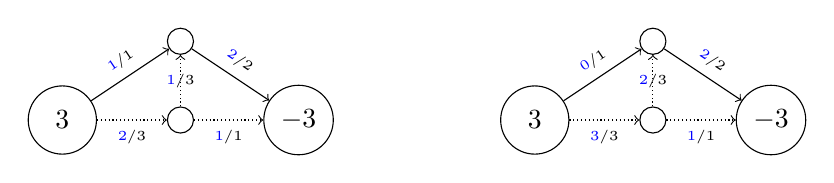
\begin{tikzpicture} [align=center]
\path (0, 0) node[circle, draw, text width=0.5cm] (v0) {$3$}
	  (1.5, 1) node[circle, draw] (v1) {}
	  (1.5, 0) node[circle, draw] (v2) {}
	  (3, 0) node[circle, draw, text width=0.5cm] (v3) {$-3$}
	  
	  (6, 0) node[circle, draw, text width=0.5cm] (v4) {$3$}
	  (7.5, 1) node[circle, draw] (v5) {}
	  (7.5, 0) node[circle, draw] (v6) {}
	  (9, 0) node[circle, draw, text width=0.5cm] (v7) {$-3$};

\draw[->] (v0) to node [sloped, anchor=center, above] {\tiny\textcolor{blue}{$1$}/1} (v1);
\draw[->] (v1) to node [sloped, anchor=center, above] {\tiny\textcolor{blue}{$2$}/2} (v3);
\draw[densely dotted, ->] (v0) to node [below] {\tiny\textcolor{blue}{$2$}/3} (v2);
\draw[densely dotted, ->] (v2) to node {\tiny\textcolor{blue}{$1$}/3}(v1);
\draw[densely dotted, ->] (v2) to node [below] {\tiny\textcolor{blue}{$1$}/1} (v3);

\draw[->] (v4) to node [sloped, anchor=center, above] {\tiny\textcolor{blue}{$0$}/1} (v5);
\draw[->] (v5) to node [sloped, anchor=center, above] {\tiny\textcolor{blue}{$2$}/2} (v7);
\draw[densely dotted, ->] (v4) to node [below] {\tiny\textcolor{blue}{$3$}/3} (v6);
\draw[densely dotted, ->] (v6) to node {\tiny\textcolor{blue}{$2$}/3}(v5);
\draw[densely dotted, ->] (v6) to node [below] {\tiny\textcolor{blue}{$1$}/1} (v7);
\end{tikzpicture}
\end{document}